
%(BEGIN_QUESTION)
% Copyright 2006, Tony R. Kuphaldt, released under the Creative Commons Attribution License (v 1.0)
% This means you may do almost anything with this work of mine, so long as you give me proper credit

Menneskelig hørsel er i sin natur ikke-lineær: for at en lyd skal oppfattes som dobbelt så høy, kreves {\it ti} ganger så høy effekt fra lydkilden. Derfor måles lydtrykk i enheten {\it desibel}: en ikke-lineær skala.

% Ingen blanklinjer er tillatt mellom linjer i en \halign-struktur!
% Jeg bruker kommentarer (%) i stedet, slik at TeX ikke feiler.

$$\vbox{\offinterlineskip
\halign{\strut
\vrule \quad\hfil # \ \hfil &
\vrule \quad\hfil # \ \hfil &
\vrule \quad\hfil # \ \hfil \vrule \cr
\noalign{\hrule}
%
% Første rad
Oppfatning & dB & Effekt \cr
%
\noalign{\hrule}
%
% Neste rad
(Grunnnivå) & 0 & (Grunnnivå) \cr
%
\noalign{\hrule}
%
% Neste rad
2 $\times$ & 10 & 10 $\times$ \cr
%
\noalign{\hrule}
%
% Neste rad
4 $\times$ & 20 & 100 $\times$ \cr
%
\noalign{\hrule}
%
% Neste rad
8 $\times$ & 30 & 1000 $\times$ \cr
%
\noalign{\hrule}
%
% Neste rad
16 $\times$ & 40 & 10000 $\times$ \cr
%
\noalign{\hrule}
%
% Neste rad
32 $\times$ & 50 & 100000 $\times$ \cr
%
\noalign{\hrule}
} % Slutt på \halign
}$$ % Slutt på \vbox

Dette er et problem dersom vi prøver å konstruere en forsterker med variabelt lydnivå, for eksempel en effektforsterker for PA-anlegg eller et Hi-Fi-system. Vi ønsker at volumknotten skal ``kjennes'' naturlig slik at hver like store rotasjonsøkning gir en tilsvarende økning i opplevd lydnivå gjennom hele området.

En audioforsterker med lineært potensiometer for volumkontroll vil ikke gi ønsket ``følelse''. I stedet vil sammenhengen mellom knotterotasjon og lyd se omtrent slik ut i et plott:

$$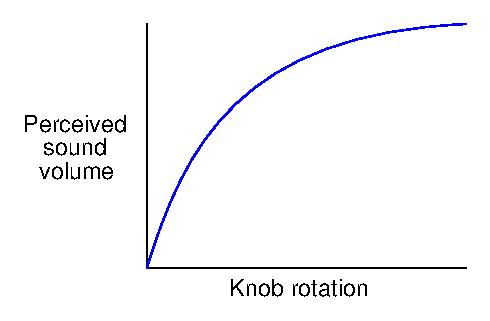
\includegraphics[width=15.5cm]{i01381x01.eps}$$

\filbreak

For å motvirke denne trenden og ``linearisere'' funksjonen mellom knotterotasjon og lyd bruker forsterkerdesignere vanligvis {\it audio-taper-potensiometre} som volumkontrollelement i kretsene. Audio-taper-potensiometre er bygget med ikke-lineære motstandsbaner innvendig, slik at spenningsdelingen bevisst ikke følger lineært med akselposisjon:

$$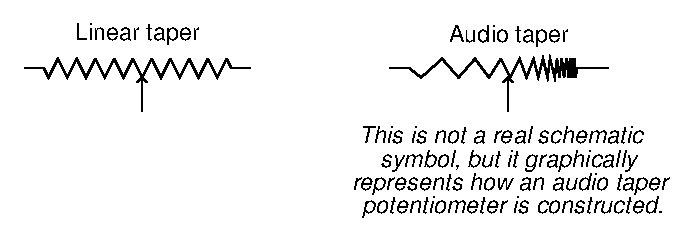
\includegraphics[width=15.5cm]{i01381x02.eps}$$

\filbreak

Hvis vi tegner spenningsdelingsforhold mot knotterotasjon for begge potensiometrene, får vi følgende resultater:

$$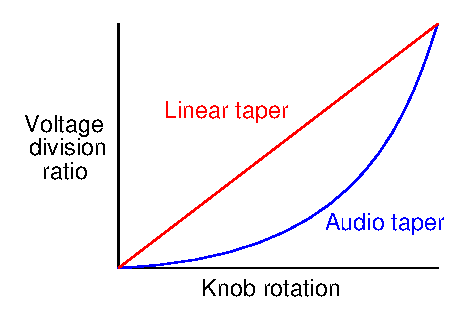
\includegraphics[width=15.5cm]{i01381x03.eps}$$

Når et slikt potensiometer brukes som volumkontroll i en audioforsterker, ``opphever'' den ikke-lineære naturen i audio-potensiometeret den naturlige ikke-lineariteten mellom effekt og opplevd lydstyrke i menneskelig hørsel. Resultatet er en mye mer lineær ``følelse'' i hvordan knotten styrer volumet.

\vskip 10pt

Nå lurer du sannsynligvis på: {\it ``Hva har dette med reguleringsventiler å gjøre?''} Analogien er som følger: den ikke-lineære naturen i menneskelig hørsel tilsvarer tendensen i prosessrør og strømningsmotstand til å ``forvrenge'' karakteristikken til en installert reguleringsventil, og audio-taper-potensiometeret oppfører seg som en equal-percentage-reguleringsventil. Forklar hvordan equal-percentage-reguleringsventiler virker for å ``linearisere'' funksjonen mellom akselposisjon og strømningsrate i en prosess.

\vskip 20pt \vbox{\hrule \hbox{\strut \vrule{} {\bf Forslag til sokratisk diskusjon} \vrule} \hrule}

\begin{itemize}
\item{} Skisser hvordan en lydsignalkilde og en lydlast (f.eks. forsterkerinngang) kobles til audio-taper-potensiometersymbolet vist med ``komprimert'' skala. Med andre ord: avgjør hvilken ende av potensiometerets faste kontakter som skal være felles for både lydkilde og lydlast.
\end{itemize}

\underbar{file i01381}
%(END_QUESTION)





%(BEGIN_ANSWER)

Jeg gir ikke bort svaret her, fordi analogien inneholder nok detaljer. Hvis du trenger mer hjelp, slå opp i en referanse om reguleringsventiler under temaene ``installed characteristic'' og ``distortion''.

\vskip 10pt

En annen analogi som kan hjelpe deg å forstå hvordan equal-percentage-ventiler virker, og som ligger nærmere reguleringsventiler enn audioforsterkere, er kvadratrotekstraksjon for nivåbaserte strømningsinstrumenter. Når vi måler væskestrøm med energivekslende primærelementer som orificeplater, venturirør og pitotrør, må vi ``kvadratrotbehandle'' differansetrykkmålingen for å gjøre den om til en strømningsmåling. Med andre ord: vi kompenserer én ikke-linearitet med en komplementær ikke-linearitet, altså en som ``opphever'' den første slik at sluttresultatet blir lineært.

%(END_ANSWER)





%(BEGIN_NOTES)

Den spesifikke ikke-lineariteten i en equal-percentage-reguleringsventil forsøker å være den inverse funksjonen av den ikke-lineære trykk-/strømningsfunksjonen i et reelt rørsystem. Vi gjør dette for å få installert karakteristikk så lineær som mulig, slik at vi får mer konsistent {\it gain} gjennom ventilens spindelvandring. Dette er viktig for stabil og konsistent regulering over et bredt område av strømningsforhold.

\vskip 10pt

Det vi faktisk ser her er en anvendelse av {\it kjerneregelen} i kalkulus:

$$\hbox{Hvis \hskip 5pt} y = f(u) \hbox{ og } u = g(x) \hbox{ slik at } y = f\left(g(x)\right) \hbox{ ,}$$

$$\hbox{Da \hskip 5pt} {dy \over dx} = {dy \over du}{du \over dx}$$

\filbreak

For audio-applikasjonen: Lydstyrke ($y$) er en funksjon av audioeffekt ($u$), og audioeffekt ($u$) er en funksjon av potensiometerstilling ($x$), slik at lydstyrke er en sammensatt funksjon av effekt og potensiometerstilling ($y = f(g(x))$). Nøkkelen til en jevn ``følelse'' i volumknotten er at den deriverte $dy \over dx$ holdes konstant. Det betyr at $dy \over du$ og $du \over dx$ må være gjensidige størrelser.

\vskip 10pt

For reguleringsventil-applikasjonen: Strømning ($Q$) er en funksjon av ventilens $C_v$, og ventilens $C_v$ er en funksjon av spindelstilling ($x$), slik at strømning er en sammensatt funksjon av $C_v$ og spindelstilling ($Q = f(g(x))$). Nøkkelen til konstant ventilforsterkning i prosessen er at den deriverte $dQ \over dx$ forblir konstant. Det betyr at $dQ \over dC_v$ og $dC_v \over dx$ må være gjensidige størrelser.

%INDEX% Final Control Elements, valve: characterization

%(END_NOTES)
